	\documentclass[
	%   draft,
	  a4paper,
	%   titlepage,
	  onecolumn,
	%  twocolumn,
	  11pt,
	  ]%
	% {scrartcl}%
	{article}%
	
	
	\usepackage[utf8x]{inputenc} 
	%\usepackage[utf8]{inputenc} % codificação deste ficheiro em UTF-8 
	
	\usepackage[T1]{fontenc}
	
	%% precisa ser carregado um outro tipo de letra por causa do efeito colateral do pacote T1:
	\usepackage{lmodern} % Fonte "Latin Modern" - A solução óptima para fontes latinas (resolve o problema do T1)
	% \usepackage{times}   % Fonte "Times"
	
	
	\usepackage{textcomp} % caracteres extra - símbolo do euro por exemplo
	
	% \usepackage[portuguese]{babel} % tradução portuguesa

	\newcommand{\referencesname}{Bibliografia}
	
	
	\renewcommand*\listfigurename{Indice de figuras}
	
	%%%%%%%%%% Packages
	
	
	\usepackage[pdftex]{graphicx} % figuras 
	
	
	%Figure side by side

	%\usepackage{subfig}
	\usepackage{graphicx}
	\usepackage{caption}
	\usepackage{subcaption}
	
	
	\usepackage{array} % mais opções nas tabelas (m{width}, b{width}, ...)
	\setlength{\extrarowheight}{1pt} % extra espaço entre as linhas das tabelas
	% \usepackage{multirow} % tabelas com células multilinha
	
	\usepackage{fancyhdr} % Estilo de página
	
		
	\usepackage[usenames,hyperref,pdftex%
	 ,svgnames%
	 ,x11names%
	 ,dvipsnames%
	%  ,cmyk
	 ]{xcolor} % Utilização de cores
	\usepackage{multicol}
	
	
	\usepackage[left=2.3cm,right=2.3cm,top=2.4cm]{geometry} % Margins
	
	
	% math packages by AMS
	\usepackage{amsmath} % main one
	
	
	

	\usepackage{fancyvrb} % more verbatim options 
	
		
	\usepackage[protrusion=true,expansion=true,stretch=10,shrink=10]{microtype} % micro-typographic extensions of pdfTEX (gets high quality text compostion)
	
	\usepackage[
	      pdftex,             %driver
	      colorlinks=true,    %no frame around URL
	      urlcolor=Black,    %no colors
	%       menucolor=black,    %no colors
	      linkcolor=black,    %no colors
	%       pagecolor=black,    %no colors
	      citecolor=Black,    %no colors
	      bookmarks=true,    %tree-like TOC
	      bookmarksopen=true,    %expanded when starting
	      bookmarksnumbered=true, %Put section numbers in bookmarks
	      hyperfootnotes=true,    %no referencing of footnotes, does not compile
	      pdfpagemode=UseOutlines,    %show the bookmarks when starting the pdf viewer
	      plainpages=false, %solve problem ``destination with the same identifier'' warning
	      pdfpagelabels %solve problem ``destination with the same identifier'' warning
	]{hyperref} % fazer hyperlinks (usar como último ``usepackage'')
	
	

	
	 \usepackage[colorinlistoftodos]{todonotes}
	
	\usepackage{xifthen}
	\usepackage{csvsimple}
	
	

	
	\newcommand{\tab}{\hspace*{2em}}
	
	%Text subscript
	\usepackage{fixltx2e}
	
	% Matrizes
	\usepackage{amsmath}
	
	%rename defaults
	
	\renewcommand{\figurename}{Figura}
	\renewcommand{\contentsname}{Indíce}
	\renewcommand{\abstractname}{Introdução}
	\renewcommand{\refname}{Referências}
	
	
	%Figure side by side
	
	
	%force float position
	\usepackage{float}
	\usepackage[section]{placeins}
	
	\makeatletter
	\AtBeginDocument{%
	  \expandafter\renewcommand\expandafter\subsection\expandafter{%
	    \expandafter\@fb@secFB\subsection
	  }%
	}
	\makeatother

	
	%Parametros de exibicao de codigo
	\usepackage{listings}
	\usepackage{color}
	
	\definecolor{mygreen}{rgb}{0,0.6,0}
	\definecolor{mygray}{rgb}{0.5,0.5,0.5}
	\definecolor{mymauve}{rgb}{0.58,0,0.82}
	
	
	
	
	%% Criação de comandos:
	\newcommand{\note}[1]{{\sffamily \slshape \textcolor{red}{#1}}}
	
	\colorlet{FPathColor}{Sepia}
	\colorlet{CmdColor}{blue}
	\colorlet{CmdRuleColor}{LightSteelBlue}
	\colorlet{FileTextColor}{DarkGreen}
	\colorlet{FuncColor}{DeepPink4}
	\CustomVerbatimCommand{\FPath}{Verb}{formatcom=\color{FPathColor},fontsize=\normalsize}
	\CustomVerbatimCommand{\Cmd}{Verb}{formatcom=\color{CmdColor},fontsize=\normalsize}
	\CustomVerbatimCommand{\FText}{Verb}{formatcom=\color{FileTextColor},fontsize=\normalsize}
	\CustomVerbatimCommand{\Func}{Verb}{formatcom=\color{FuncColor},fontsize=\normalsize}
	\DefineVerbatimEnvironment%
	  {Command}{Verbatim}
	  {formatcom=\color{CmdColor},frame=single,rulecolor=\color{CmdRuleColor},fontsize=\normalsize}
	\DefineVerbatimEnvironment%
	  {FileText}{Verbatim}
	  {formatcom=\color{FileTextColor},fontsize=\normalsize}
	
	
	% % Authors:
	
	
	
	\newcommand{\MYauthor}{Luís Rocha} 
	\newcommand{\MYnumber}{2010127532}
	
	\newcommand{\MYauthorII}{José Medeiros}
	\newcommand{\MYnumberII}{2010129934} 
	
		
	% % Titles:
	\newcommand{\MYtitle}{ROS - Detector de metais}
	\newcommand{\MYsubtitle}{Projecto} % Can be empty
	
	
	% % Course
	
	\newcommand{\MYcoursename}{Mecatrónica}
	\newcommand{\MYcourseyear}{2013/2014}
	
	
	% % PDF infos
	
	\newcommand{\MYkeywords}{} % Can be empty
	\newcommand{\MYsubject}{} % Can be empty
	
	
	%% Document format
	
	%% Fancy Headers
	\lhead{
\includegraphics[width=2cm]{logo_deec.pdf}}
	\chead{\sc\footnotesize Universidade de Coimbra\\
	Faculdade de Ciências e Tecnologia\\
	Departamento de Engenharia Electrotécnica e de Computadores}
	\rhead{
\includegraphics[width=0.8cm]{logo_fctuc.pdf}}
	\setlength{\headheight}{43pt}
	
	% Title
	\title{{\large\MYcoursename\ -- \MYcourseyear}\\[2mm]
	{\MYtitle}
	\ifthenelse{\equal{\MYsubtitle}{}}
	{\vspace*{1mm}}   {\\{\large\MYsubtitle}\vspace*{1mm}}
	}
	
	% Author / Number
	\author{%
	\MYauthor\\{\normalsize \href{mailto:ze_pedrom@hotmail.com}{\MYnumber}}
	\ifthenelse{\isnamedefined{MYauthorII}}
	{\and\MYauthorII\\{\normalsize \href{mailto:luis.rocha.jacinto@gmail.com}{\MYnumberII}}}    {}
	\ifthenelse{\isnamedefined{MYauthorIII}}
	{\and\MYauthorIII\\{\normalsize \href{mailto:a\MYnumberIII@alunos.deec.uc.pt}{\MYnumberIII}}}   {}
	}
	
	% Version / Date
	\date{%
	% \normalsize \today
	\mbox{}
	}

      
	
	
	%% PDF definitions:
	
	\hypersetup{%
	   pdftitle=\MYtitle,%
	   pdfauthor=\MYauthor,%
	%    pdfcreator=,%
	   pdfkeywords= {\MYkeywords},%
	%    pdfproducer=,%
	   pdfsubject= \MYsubject%
	} % informações do pdf (pacote hyperref)
	
	\pdfinfo{
	/Title	(\MYtitle)
	/Author (\MYauthor)
	/Keywords (\MYkeywords)
	} % informações do pdf
	
	\graphicspath{ {img/} } % Pasta das Imagens
	
	

	
	
	
	\begin{document}
	
	\maketitle
	\thispagestyle{fancyplain}
	
	\setlength{\parskip}{10pt}
	% Introdução
	 \begin{abstract} % (optional)
	
	 
	\tab Neste trabalho foi incorporado um sensor indutivo ao robô Roomba para a detecção de minas terrestres através do uso de ROS.
	Para o controlo do robô foi necessário fazer uso de um API\cite{apiroomba} que permitisse a comunicação com o mesmo e a plataforma ROS. Com este foi possível controlar os movimentos
	do robô através do teclado usando um terminal.\\
	\tab Quando na presença de metais e usando os dados devolvidos pelo sensor - proximidade e frequência - é possivel determinar se o robô se encontra perante uma mina.
	Com base neste princípio é possível detectar a presença de minas.

	\end{abstract}
	
	  	

	
	\begin{figure}[ht]
	  \centering
	  \begin{subfigure}{0.4\textwidth}
	    \centering
	    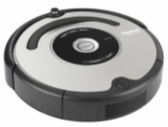
\includegraphics[width=36mm,scale=0.1]{robot_roomba.png}
	    \caption{Robot Roomba}
	    \label{fig:robot_roomba}
	  \end{subfigure}%
	  \begin{subfigure}{0.6\textwidth}
	    \centering
	    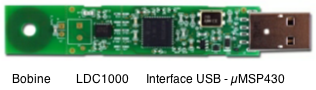
\includegraphics[width=82mm,scale=0.9]{ldc_specs.png}
	    \caption{Componentes do LDC100EVM}
	    \label{fig:ldc_specs}
	  \end{subfigure}
	  
	  \caption{Roomba e LDC100EVM com os componentes}
	  \label{fig:romba_ldc}
	  \end{figure}
	  
	
	  
	
	
	
	%\newpage
		
	
	%\listoftodos
	
	\newpage
	
        \tableofcontents

        \newpage
	
	\listoffigures

	\newpage
	
	\section{Lista de acrónimos}
	
	
	\begin{description}
	    \item[ROS] \hfill \\
	     Robot Operation System - Sistema Operativo para Robos
	   \item[LRC Meter] \hfill \\
	   Aparelho que mede indutância, capacitância e resistência de um componente\cite{lrc}
	   \item[PCB] \hfill \\
	   Printed Circuit Board - Placa de Circuito Impresso
	   \item[API] \hfill \\
	   Aplication Programming Interface - Interface de Programação de Aplicações
	   \item[USB] \hfill \\
	   Universal Serial Bus
	   \item[VNC] \hfill \\
	   Virtual Network Computing
	\end{description}
      

      
	
	
	\section{Material disponível}
	
	
	
		
	\begin{description}
	  \item[Computadores] \hfill
	  \begin{description}
	    \item Notebook
	    \item Netbook
	  \end{description}
	  \end{description}
	  
	  \begin{description}
	  \item[Componentes/Aparelhos Electrónicos] \hfill
	  \begin{description}
	  \item Bobine de 1.71 mH 
	  \item Condensador de 3.09 nF
	  \item LRC Meter - Modelo 186
	  \end{description}
	  \end{description}
	  
	  
	  \begin{description}
	  \item[Robô Detector de Minas] \hfill
	  \begin{description}
	  \item Robô Roomba 555
	  \item Detector de Metais - LDC1000EVM
	  \item Api/Wrapper para comunicação com o Romba
	  \end{description}
	  \end{description}
	  

 	  
	
	\begin{description}
	  \item[Acessórios] \hfill
	  \begin{description}
	    \item Teclado Wireless
 	  \item USB Hub com quatro portas 
	  \end{description}
	  \end{description}

	
	
	
	
	\newpage
	
	\section{Descrição do problema}
	
	\tab Pretende-se detectar minas terrestres através do uso de um robô Roomba e de um sensor indutivo LCD1000EVM capaz de medir
	a proximidade e a frequência associada á presença de um metal nas imediações. 
	Este sensor é composto por uma bobine em PCB, um LDC1000 que faz uso da bobine e um microcontrolador - MSP430, tal como se pode observar na
	figura \ref{fig:ldc_specs}. \\
	\tab Para ser possivel a concretização deste projecto é necessário implementar uma interface de comunicação entre
	o computador e o sensor para a aquisição de dados. Esta interface vai ser baseada num protocolo de comunicação que terá
	que ser o mesmo que é usado pelo microcontrolador. Será portanto necessário entender bem o protocolo visto que toda a base
	deste projecto se baseia neste sensor. \\
	\tab Após a interligação entre o sensor e o computador através de uma porta USB é necessário combinar o robô Roomba com o sensor utilizando a plataforma ROS \footnote{Distribuição Hydro}.
	Para isso é obrigatório fazer uso de transformadas ($tf's$) para referenciar o sensor ao eixo/referencial em relação ao referencial principal do robô. Mais á frente no relatório explicaremos melhor o conceito
	e a maneira como interligamos as transformações na nossa implementação
	Este passo é importantissimo para que se possa calcular as posições onde o sensor detecta minas.

	
	\section{Conhecimentos necessários}

	
	\tab Após analisarmos os requisitos deste projecto chegámos á conclusão de que era necessário familiarizarmos
	com a plataforma ROS. Sendo assim seguimos os tutoriais existentes no website WikiRos\cite{wikiros}.
	Após concluidos os tutoriais, ficamos aptos a usar ROS usando C++ como linguagem de programação. \\
	\tab Os seguintes conceitos/utilidades foram usados no nosso projecto, a sua explicação breve apresenta-se
	abaixo:
	
	\begin{description}
	    \item[Tf] \hfill \\
	  Estruturação dos referenciais do robô assim como as transformações necessárias entre os diferentes componentes \footnote{Sensores, plataformas, rodas, entre outros} do robô para que se possa saber as posições de qualquer elemento num dado instante. 
	    \item[Marker] \hfill \\
	  Estrutura de dados que permite usar as bibliotecas do \textit{rviz} para marcar minas no mapa. A posição das minas é obtida pela transformação da \textit{tf} do sensor em relação ao referencial base do robô.
	    \item[ArrayMarker] \hfill \\
	  Guardamos os markers (minas) que detectamos num array de markers. Para tal é necessário fazer \textit{push\_back} de um marker para o array quando é detectada a presença de uma mina.
	     \item[Serial Port] \hfill \\
	  Protocolo de comunicação usado para comunicar com o sensor através de uma porta USB.
	\end{description}
      

	
	\section{Solução proposta}
	
	
	\subsection{Hardware}
	
	 
	 Como podemos ver na figura \ref{fig:circuito4}, foi colocado numa breadboard o condensador e foram feitas as ligações necessárias de modo a facilitar
	a mudança de bobines e para garantir que o circuito está em contacto com os componentes. Foi ainda soldado ao sensor dois fifos conectores para tornar mais fácil o seu uso.
	
	
	
	
	
	\begin{figure}[ht]
	\centering
	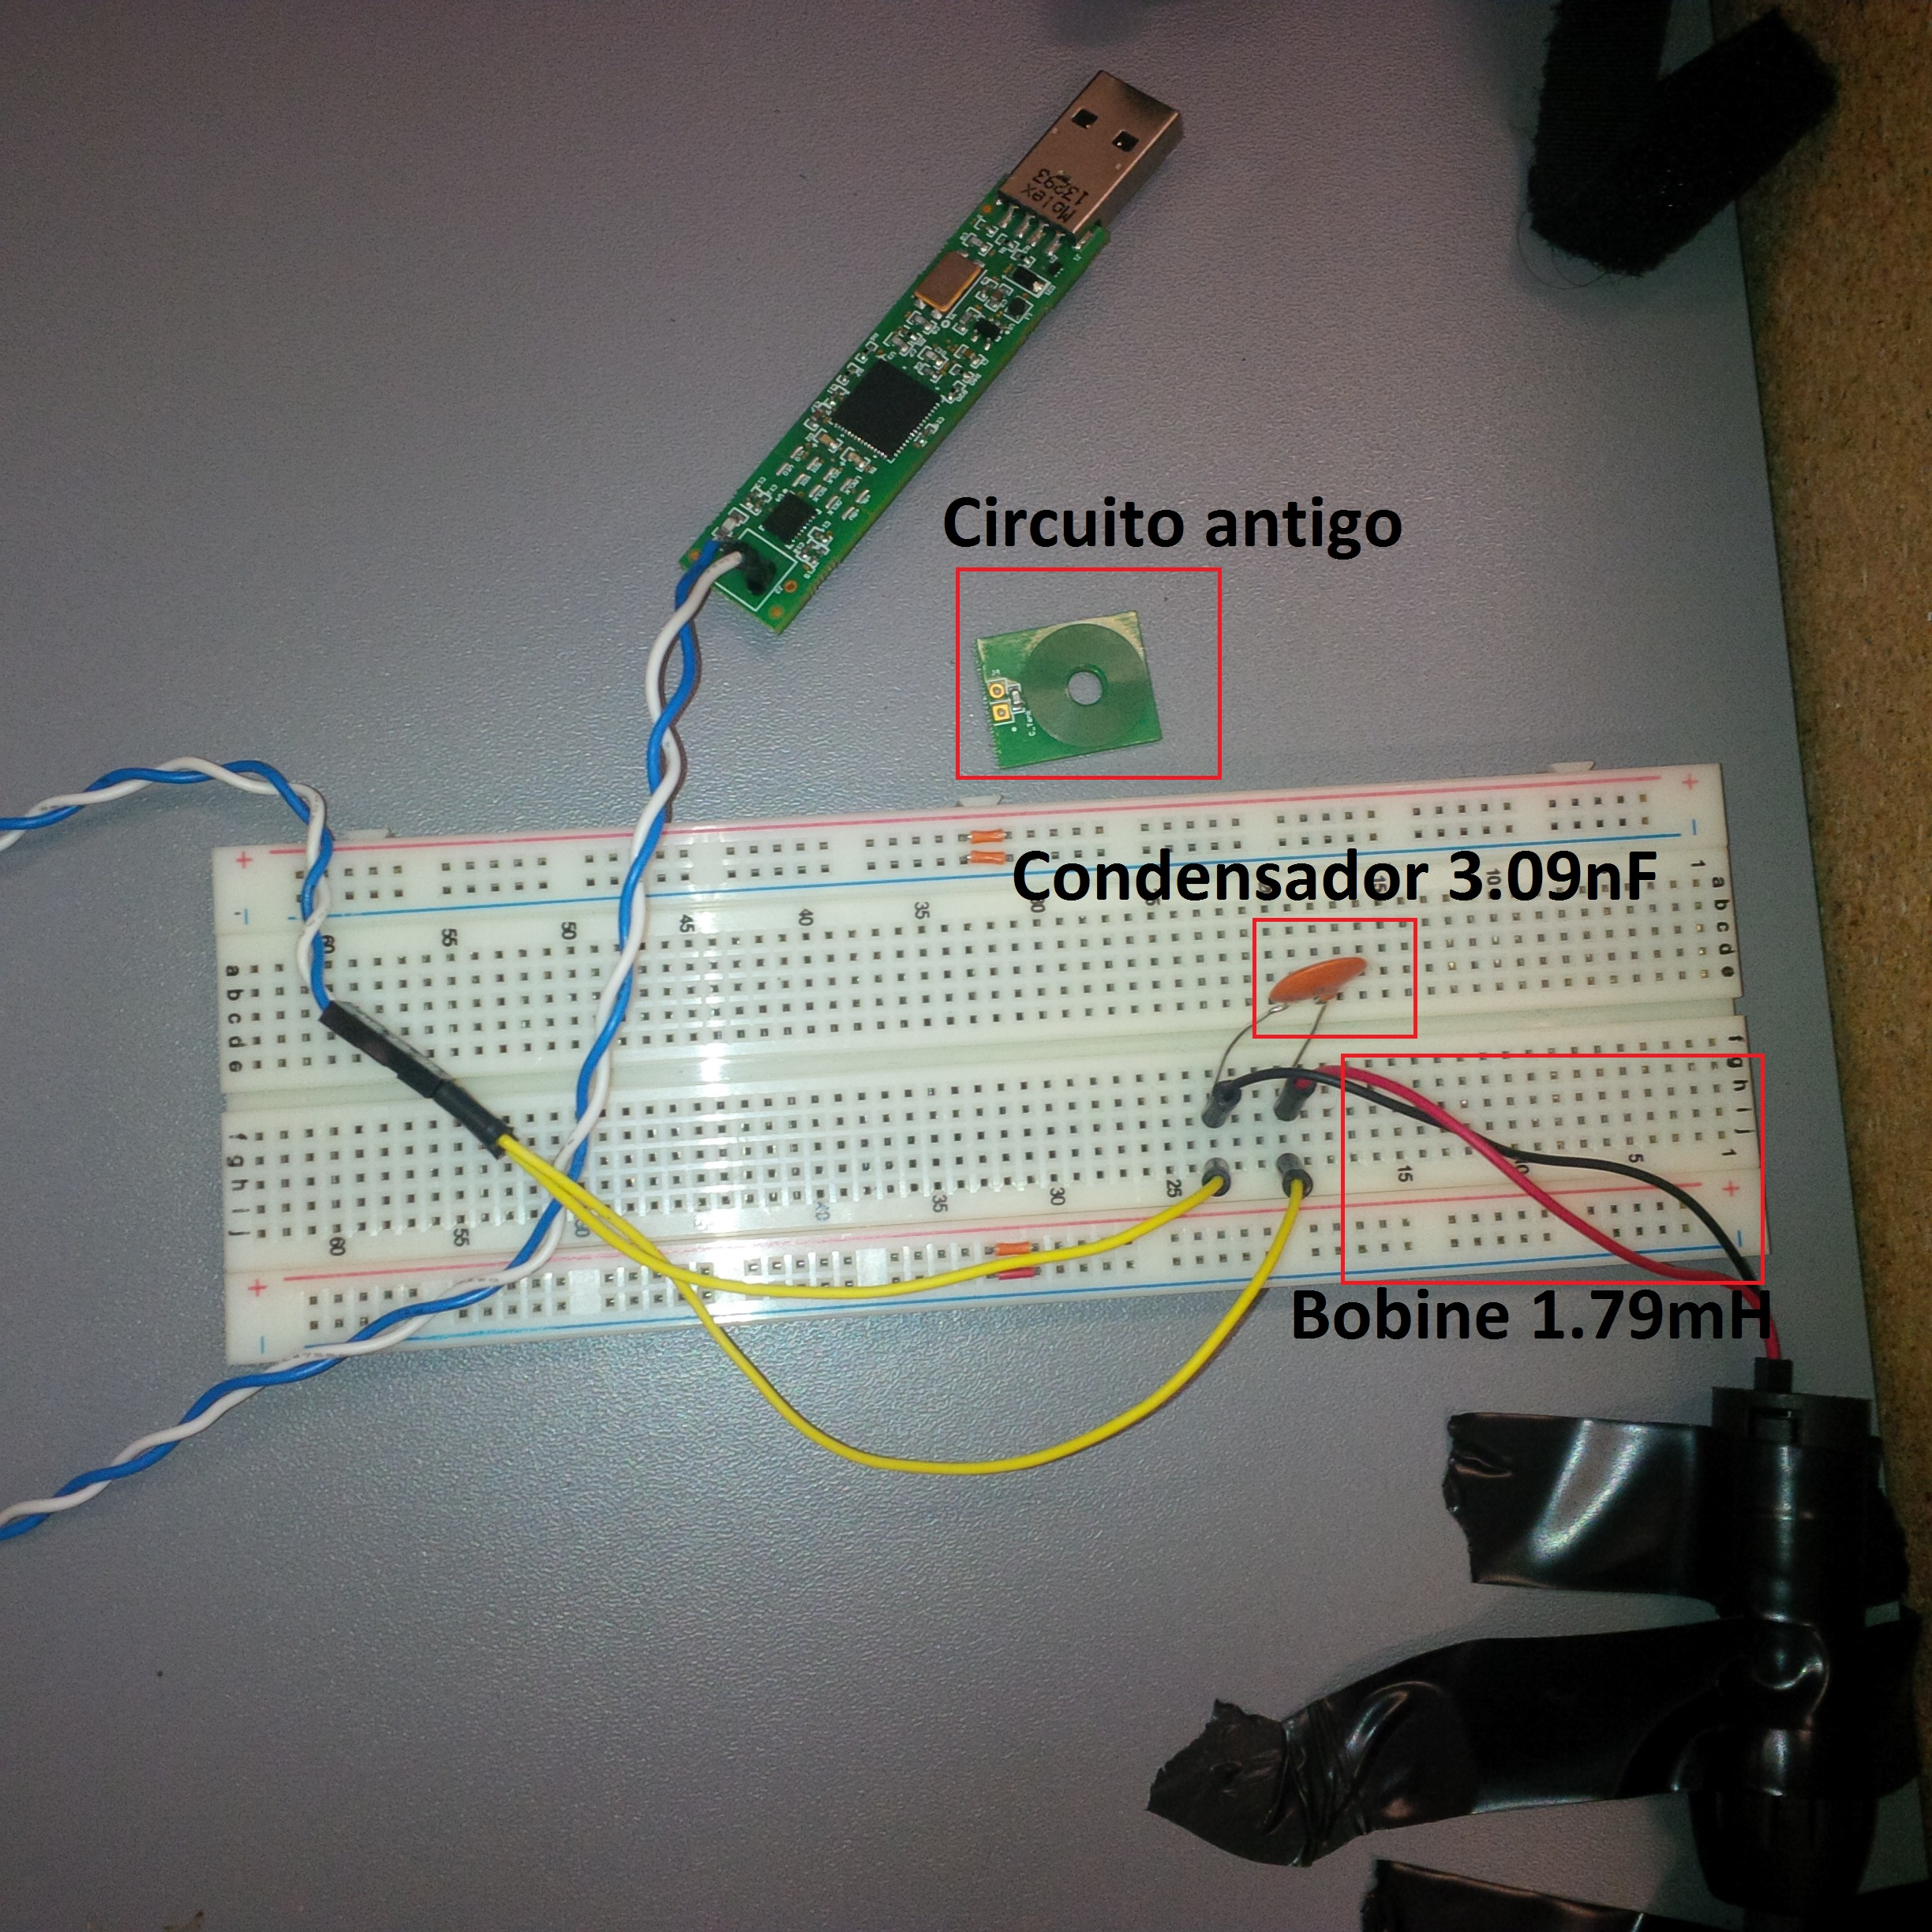
\includegraphics[width=80mm,scale=0.7]{circuito4.jpg}
	\caption{Placa breadboard + Sensor }\label{fig:circuito4}
	\end{figure}
	
	Em termos de ligações é mais facil de compreender na figura \ref{fig:roomba2},
	onde é possivel ver a ligação dos componentes ao Roomba e ao sensor. O computador vai comunicar com o Roomba e receber dados do sensor.
	Através da plataforma ROS é feito o controlo do Roomba por teclado e feita a interligação dos dados enviados pelo sensor e o robô. 
	
	\begin{figure}[ht]
	\centering
	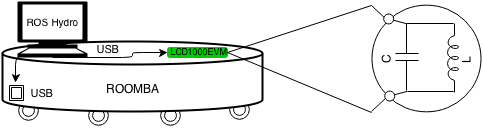
\includegraphics[width=120mm,scale=0.7]{roomba.png}
	\caption{Estrutura do robô Roomba com o sensor LDC100EVM }\label{fig:roomba2}
	\end{figure}
	
	\newpage
	
	
	
	
	
	\subsubsection{Introdução ao sensor}
	
	
	\tab O LDC100EVM é um sensor indutivo que permite medir a presença de metais retornando duas variavéis: posição do metal e a frequência de oscilação.
	É um circuito integrado que contém um microcontrolador MSP430 que é usado para fazer a interface entre
	o LDC (sensor) e um computador. 
	Este integrado vêm com uma bobine que pode ser mudada se se partir a PCB na zona a tracejado e colocando
	ai uma bobine á nossa escolha. É possivel ver na figura \ref{fig:sensor} a zona a tracejado:
	
	\begin{figure}[ht]
	\centering
	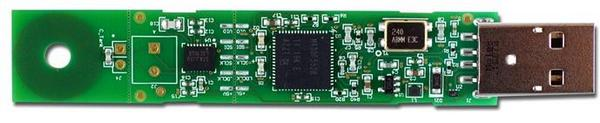
\includegraphics[width=85mm,scale=0.3]{im1.JPG}
	\caption{Sensor LDC1000EVM}\label{fig:sensor}
	\end{figure}
	
	
	
	
	
	Para dimensionar a bobine é necessário satisfazer duas condições para que o sensor possa funcionar na gama ideal:
	
	
	\begin{enumerate}
	  \item A frequência de ressonância deve estar compreendida entre 5 kHz e 5 MHz
	  \item A resistência de ressonância\footnote{Simboliza as perdas associadas ás correntes de Eddy} deve estar compreendida entre 798$\Omega$ e 3.93 M$\Omega$
	\end{enumerate}

	
	
	
	
	Para o cálculo da frequência e a respectiva resistência usa-se as seguintes fórmulas:
	
	\begin{multicols}{2}
	
	\begin{equation}\label{freq_ress}
	 f_\text{ressonância} = \frac{1}{2\pi\sqrt{LC}}
	\end{equation}
	
	\begin{equation}\label{r_ress}
	 R_p = \frac{1}{R_s} \frac{L}{C}
	\end{equation}	

	\end{multicols} 
	
	

	
	
	
	
	Abaixo encontra-se representado o esquemático do circuito que dá origem ás equações \eqref{freq_ress} e \eqref{r_ress} acima descritas:
	
	
	
	
	\begin{figure}[ht]
	  \centering
	  \begin{subfigure}{0.5\textwidth}
	    \centering
	    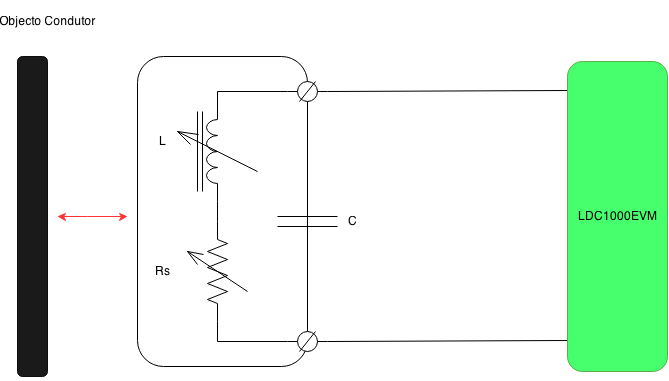
\includegraphics[width=75mm,scale=0.9]{circuito1.png}
	    \caption{Circuito físico}
	    \label{fig:roomba3}
	  \end{subfigure}%
	  \begin{subfigure}{0.5\textwidth}
	    \centering
	    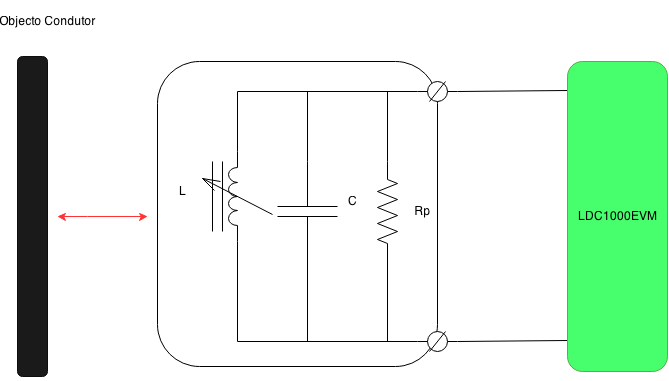
\includegraphics[width=75mm,scale=0.9]{circuito2.png}
	    \caption{Circuito simplificado}
	    \label{fig:roomba4}
	  \end{subfigure}
	  
	  \caption{Esquemático do sensor}
	  \label{fig:romba_ldc_2}
	  \end{figure}
	
	É importante referir que o circuito presente na figura \ref{fig:roomba3} é o circuito real do sensor e o da figura \ref{fig:roomba4} é uma simplificação
	que em termos prácticos permite ao sensor variar a sua gama de funcionamento afinado o valor minimo e máximo de R\textsubscript{p}. Este processo faz com que
	o sensor possa discriminar diferentes tipos de metal se bem afinado e projectado.	
	
	
	
	\subsubsection{Arquitectura}

	\tab Em termos de hardware para este trabalho foi utilizado um computador que vai controlar o Roomba e o sensor LCD1000EVM.
	No sensor foi ainda substituída a bobine por uma bobine e um condensador de valores por nós pretendidos. \\
	\tab O robô Roomba encontra-se conectado por usb a um computador que o controla através do teclado.
	Este computador encontra-se ainda ligado a um sensor LCD1000EVM que por sua vez tem ligado a si uma bobine e um condensador por nós projectados e adaptados.\\
	\tab Na figura \ref{fig:robo} é vísivel o robô já adaptado à nova bobine. Foi necessário criar uma estrutura que suportasse a bobine mas que mantivesse a estabilidade do robô,
	para tal é necessário o uso de contra-pesos como é vísivel.
	
	\begin{figure}[ht]
	\centering
	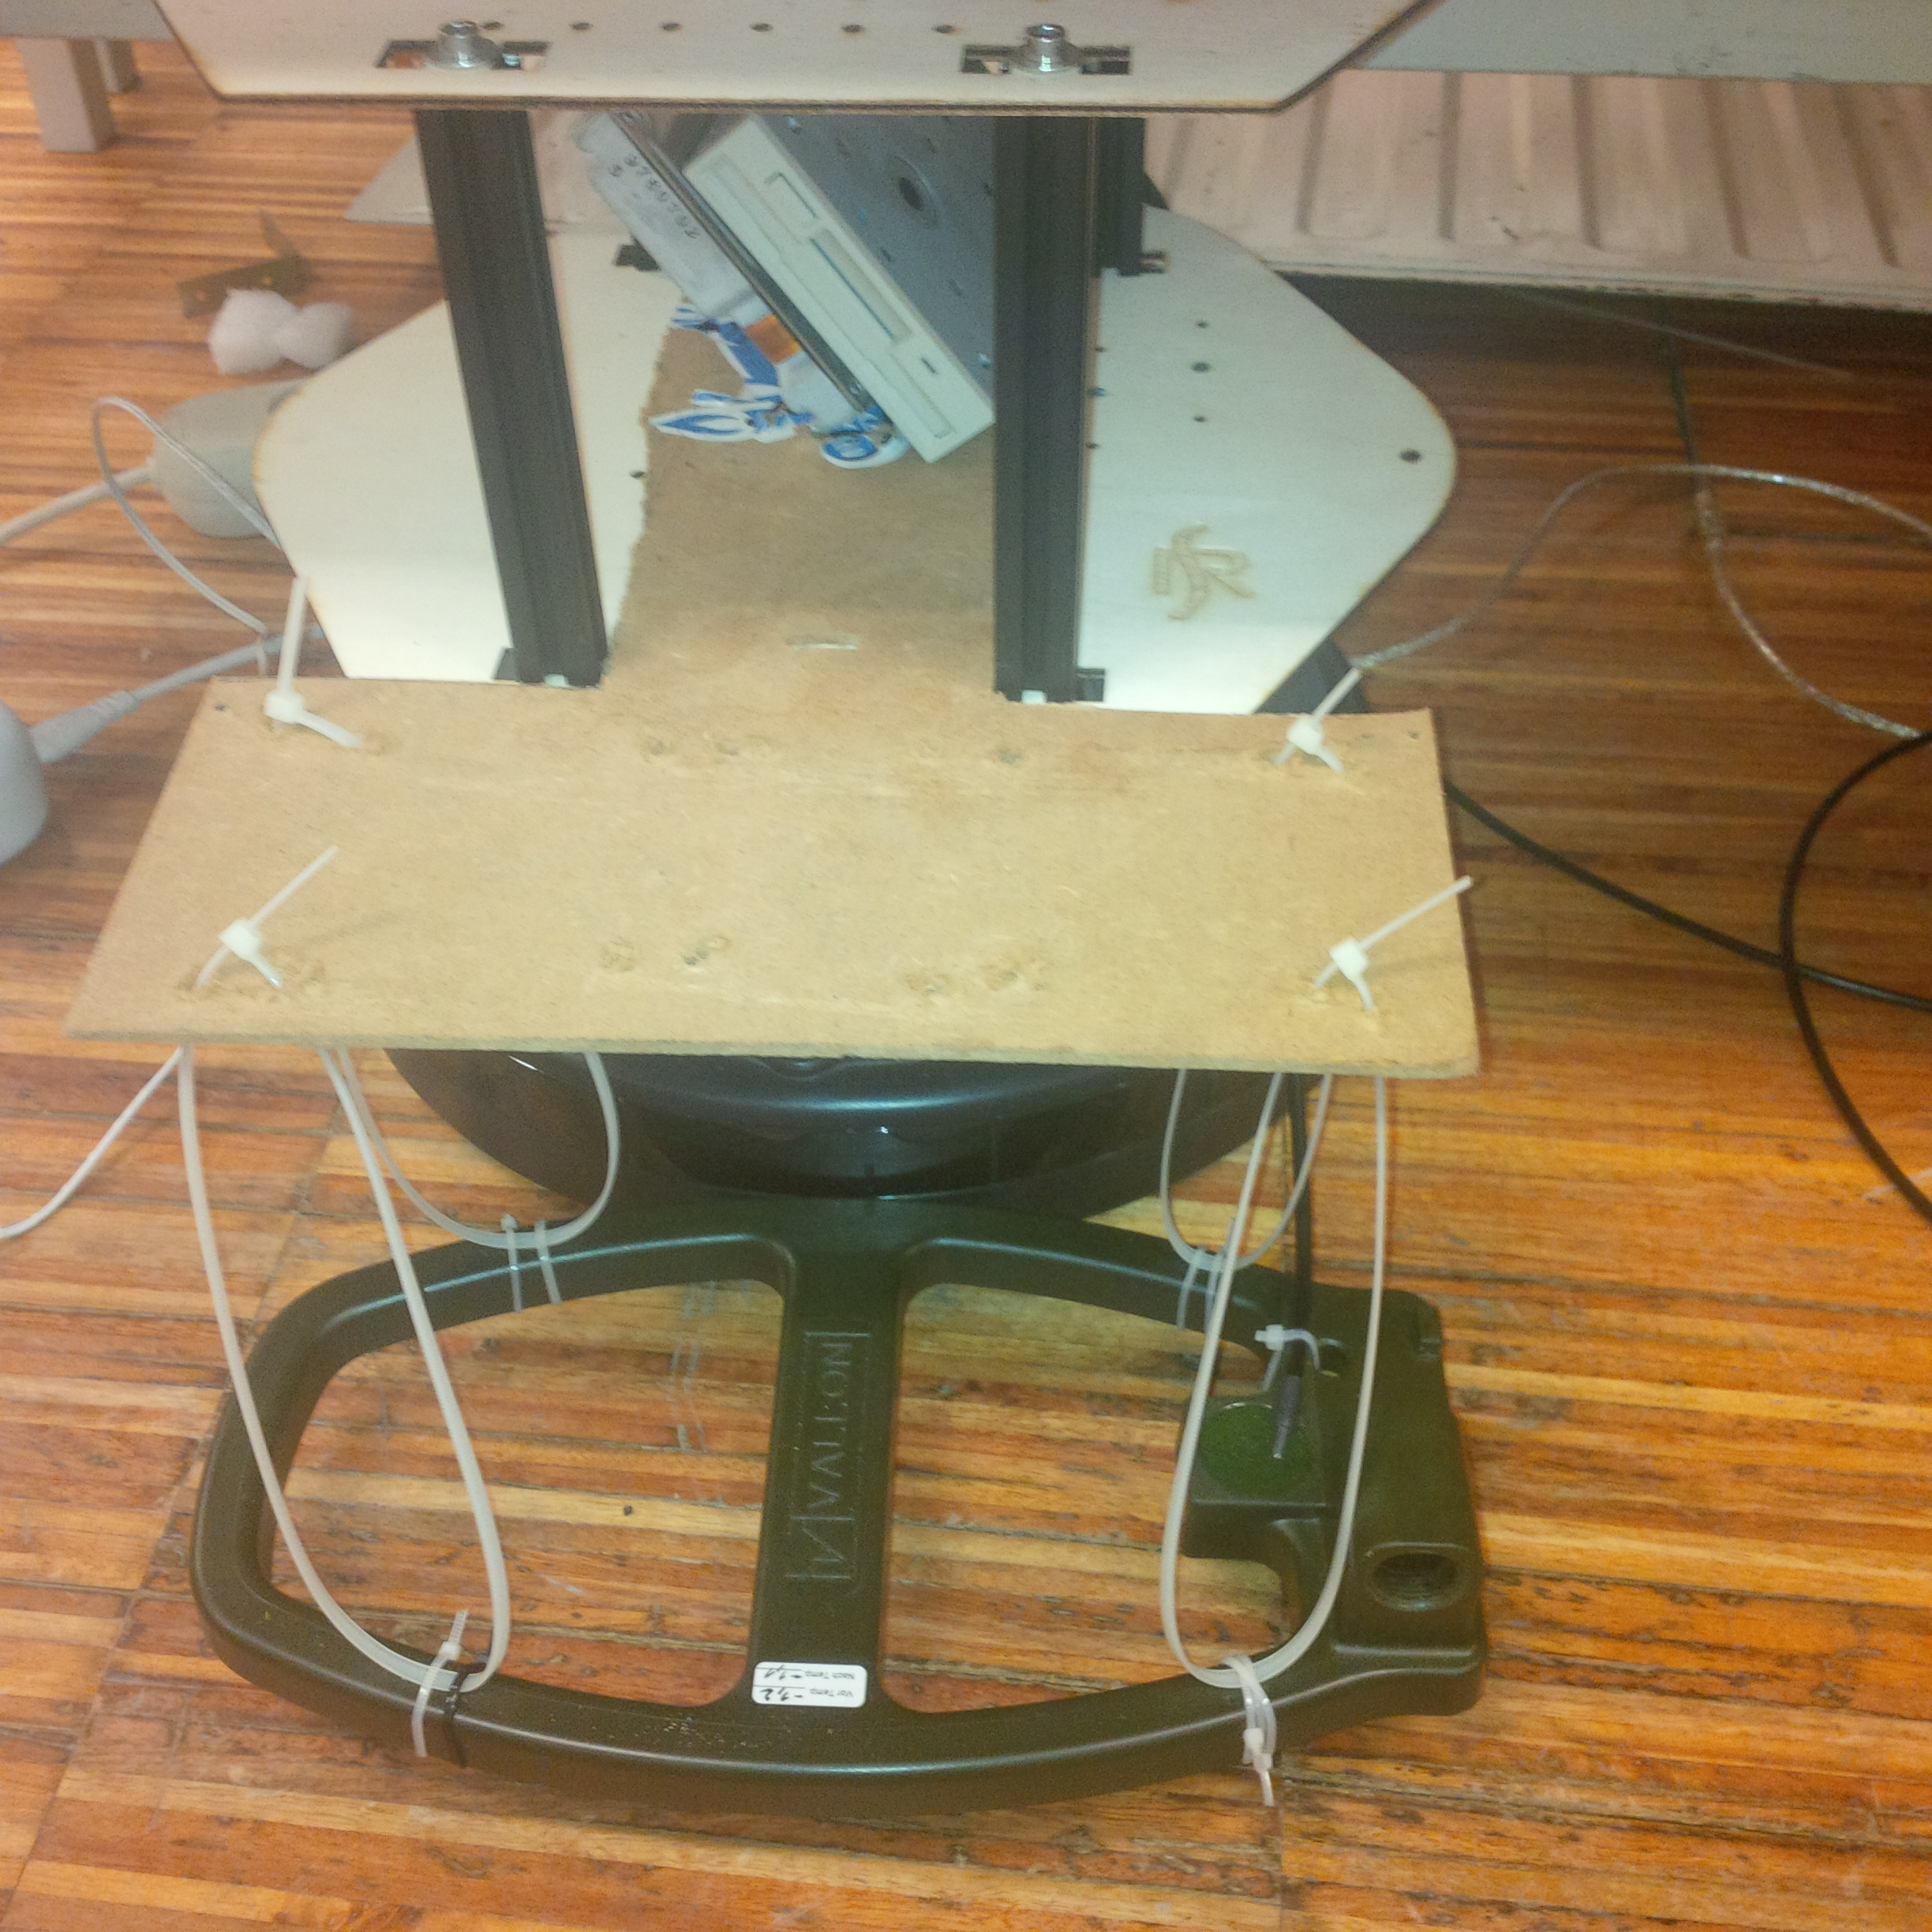
\includegraphics[width=100mm,scale=0.7]{circuitom.jpg}
	\caption{Imagem real do robô}\label{fig:robo}
	\end{figure}
	 Na figura \ref{fig:robo} é vísivel o robô já adaptado à nova bobine. Foi necessário criar uma estrutura que suportasse a bobine mas que mantivesse a estabilidade do robô,
	para tal é necessário o uso de contra-pesos como é vísivel.\\
	\tab A estrutura que suporta a bobine é facilmente removível estando apenas presa por abraçadeiras. Esta estrutura garante tanto a estabilidade do robô como da bobine.
	A bobine encontra-se ligada em paralelo ao condensador e ao sensor numa
	breadboard algo que pode ser visto na figura \ref{fig:circuito4}.
	
	
	
	
	
	\newpage
	
	
	  
	
	
	
	

	\subsubsection{Implementação}
	Como foi anteriormente explicado,  o circuito pode ser alterado e dimensionado para se trabalhar na gama de valores desejada. A seguir iremos explicar os passos necessários para implementar o novo circuito e adaptá-lo ao sensor.
	\setlength{\parskip}{10pt}
	
	\begin{enumerate}
	  \item O primeiro passo será escolher simplesmente a nova bobine por nós pretendida e escolher um condensador que permita cumprir as condições impostas à frequência de ressonância\eqref{freq_ress} e à resistência de ressonância\eqref{r_ress}.
	  \item O próximo passo será com o auxílio de um ``LCR meter'', colocando as pontas deste medidor em paralelo com o paralelo do condensador e da bobine que escolhemos têmos que anotar o valor da resistência $R_p$ lido no medidor, na ausênsia 
	  de qualquer objecto magnético.
	  \item Neste passo temos que colocar um objecto magnético o mais próximo possível da bobine e anotar o novo valor de $R_p$.
	  \item É necessário anotar também a frequência de varrimento que se encontra definida no medidor.
	  \item No passo seguinte é necessário actualizar os registos do sensor para que se adapte ao novo circuito. Para modificar os registos é necessário conectar o sensor a um computador coondutoresm windows e utilizando a gui application fornecida pela texas instruments
	  na secção de alteração dos registos terêmos que modificar três registos. O valor do registo ${R_p}_{MAX}$ deve ser alterado para o dobro do valor anotado na ausência de objectos c, como os valores disponíveis são discretos deve ser escolhido
	  o mais próximo deste valor por excesso. O valor do registo ${R_p}_{MIN}$ deve ser alterado para metade do valor anotado na presença de um objecto condutor, como os valores disponíveis são discretos deve ser escolhido
	  o mais próximo deste valor por defeito. O registo da freqûencia deve ser alterado para no máximo $80\%$ do valor da frequência de varrimento. 
	  \item Por fim é necessário partir o sensor onde diz ``coil perfuration'' na figura \ref{fig:roomba5} e soldar o paralelo da bobine e do condensador no sítio onde diz ``conections for custom LC tank'' na  figura \ref{fig:roomba5}.
	 
	\end{enumerate}

	\begin{figure}[ht]
	\centering
	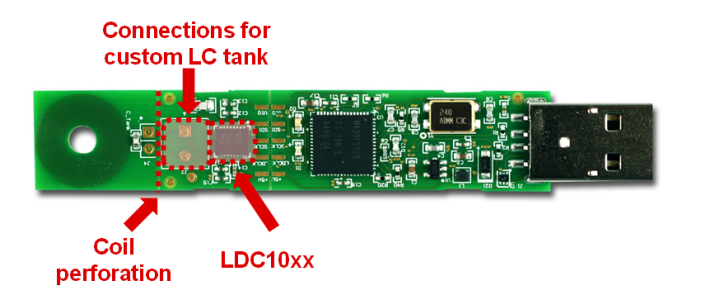
\includegraphics[width=70mm,scale=0.6]{circuito3.png}
	\caption{LCD1000EVM com indicação das perfurações}\label{fig:roomba5}
	\end{figure}
	
	\newpage
	Com o auxílio do medidor LCR meter figura \ref{fig:LCR} conseguimos adaptar o sensor à nova bobine. Para cumprir o primeiro passo referido anteriormente, primeiro medimos a indutância da nova bobine e de seguida escolhemos
	um condensador e medimos a sua capacitância.
	
	\begin{figure}[ht]
	\centering
	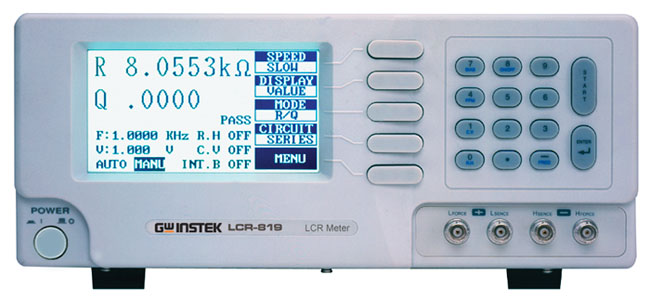
\includegraphics[width=70mm,scale=0.3]{LCR.jpg}
	\caption{LCR Meter 186}\label{fig:LCR}
	\end{figure}
	
	
	
	 Medimos o condensador e a bobine utilizando o aparelho da figura \ref{fig:LCR} obtendo 3.09 nF 
	e 1.71 mH. De seguida, utilizando \eqref{freq_ress} calculámos a nova frequência de ressonânica e obtivemos:
	
	\begin{equation}\label{freqr}
	 f_\text{ressonância} =\frac{1}{2\pi\sqrt{1.7098\times10^{-3}\times3.0863\times10^{-9}}}=69.283 kHz
	\end{equation}
	
	Como podemos concluir, a a frequência calculada está dentro da gama pretendida. 
	
	
	De seguida anotámos o valor de $R_p$ na ausência e na presença de objectos condutores obtendo
	os seguintes valores respectivamente 18.29 k$\Omega$ e 8.79 k$\Omega$. Para a obtençã destes valores
	foi usada uma frequência de varrimento de valor 66.667 kHz.
	
	
	Garantimos assim que também a resistência de ressonância se encontra dentro da gama de valores do referidos anteriormente.
	Por fim, fizémos a alteração dos registos do sensor para se adaptar aos novos valores, pelo que foram modificados os seguintes registos:
	\begin{figure}[ht]
	\centering
	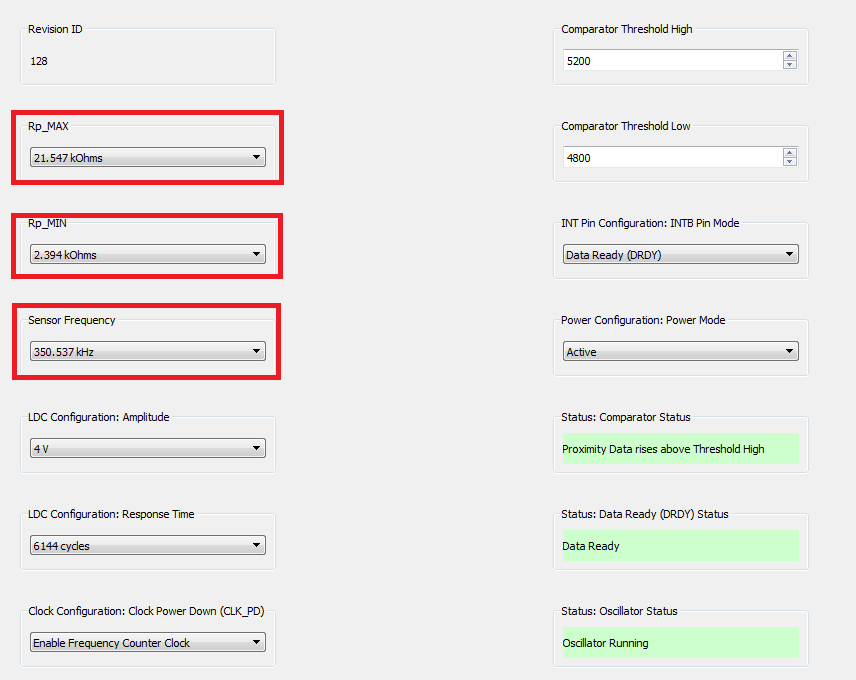
\includegraphics[width=100mm,scale=0.3]{registos.png}
	\caption{Registos do sensor LDC1000EVM}\label{fig:registos}
	\end{figure}
	
	
	\begin{enumerate}
	 \item ${R_P}_{MAX}$ foi alterado para 38.785 k$\Omega$ , valor que foi aproximado por excesso como era exigido.
	 \item ${R_P}_{MIN}$ foi alterado 4.309 k$\Omega$, valor que foi aproximado por defeito como era exigido.
	 \item Sensor frequency foi alterado para 52.231 kHz , valor que foi aproximado para o valor mais próximo de $80\%$ da frequência de varrimento, por defeito.
	\end{enumerate}
	
	Os registos que foram alterados encontram-se a vermelhor na figura \ref{fig:registos}.
Com todos os passos cumpridos o novo sensor ficou pronto a ser utilizado.

	
	
	


	\subsection{Software}
	
	\subsubsection{Como executar}
	
	Em termos de aplicação ROS, elaboramos dois tipos de programas. O primeiro contêm um nó que lê valores do sensor e publica esses dados
	usando mensagens e um outro nó que recebe esses dados e imprime para o ecrã. O segundo usa um ó que publica os dados por mensagens e um outro nó
	recebe esses dados e analisa se se trata de uma mina e em caso afirmativo marca-a num mapa desenhando um cubo de pequenas dimensões na posição em que detectou a mina.
	Abaixo encontram-se os passos necessários para os executar:
	
	
	
	

	 Primeiro Codigo:
	  	
	  \begin{enumerate}
	  \item roscore
	  \item rosrun sensor le\_sensor treshold(int)
	  \item rosrun sensor recebe\_dados
	  \end{enumerate}
	
	Segundo Codigo:
	
	\begin{enumerate}
	 \item roscore
	 \item roslaunch roomba\_bringup roomba\_555.launch
	 \item roslaunch sensor sensor.launch
	 \item rosrun sensor le\_sensor treshold (int)
	 \item rosrun sensor points\_sensor
	 \item roslaunch roomba\_teleop keyboard\_teleop.launch
	 \item rosrun rviz rviz \hfill
	\end{enumerate}


	No parametro Treshold(int) é preciso colocar um inteiro que funcionará como comparador. Quanto á configuração do rviz é necessário 
	carregar o modelo do robot, as $tf's$, os markers e o array de markers. Para poder executar correctamente o programa é
	necessário fazer sudo chmod 777 /dev/ttyUSB0 e sudo chmod 777 /dev/ttyACM0 para garantir que conseguimos abrir a porta série do Roomba
	e do sensor. 
	
	\subsubsection{Estrutura do Código}
	
	Como é possivel observar na figura \ref{fig:estrutura_codigo}, o código principal que é executado interliga-se entre os diferentes programas e o Roomba da 
	seguinte maneira:
	
	\begin{figure}[ht]
	\centering
	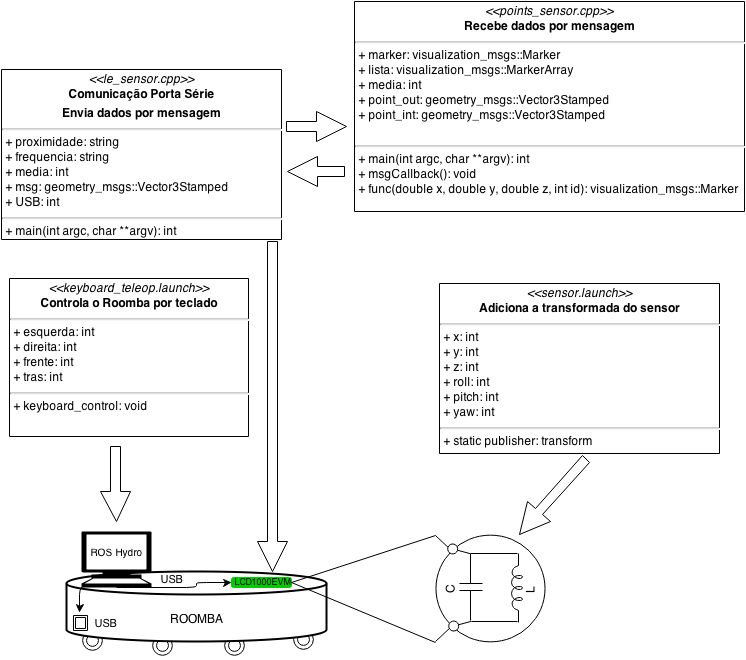
\includegraphics[width=140mm,scale=1]{estrutura_codigo.png}
	\caption{Interlicação dos diferentes programas}\label{fig:estrutura_codigo}
	\end{figure}
	
	Em termos prácticos o ficheiro \textbf{le\_sensor.cpp} comunica co o sensor por porta série e publica 
	os dados numa variavel predefinida no ROS, mensagens do tipo geometry\_msgs::Vector3Stamped.
	O ficheiro \textbf{point\_sensor.cpp} sempre que é publicado alguma mensagem com o frame\_id sensor é
	recebida calcula-se a posição do sensor no mapa virtual e verifica-se se está na presença de uma mina.
	O ficheiro launch \textbf{sensor.launch} é uma transformação do sensor em relacão é transformada odom (odometria).
	Como o sensor não apresenta nem possibilidade de translação nem rotação podemos simplesmente fazer um
	static transform publisher\cite{statictransform}. Para comandar o Roomba é usado o ficheiro launch
	\textbf{keyboard\_teleop.launch}, que contém a velocidade linear e a velocidade de rotação default. Este launcher 
	exeuta um executalvel que lê do  terminal as setas do teclado e sendo assim é possivel comandar/deslocar
	o robo.
	
	
	
	  
	
      \subsubsection{Utilização do ROS}

	\tab Utilizámos o Robot Operating System (ROS) como plataforma de comunicação entre os dois periféricos por nós utilizados e o computador.
	Com o ROS é possível implementar bibliotecas de cliente ROS como roscpp, rospy ou roslisp. Por outras palavras significa que facilmente se 
	consegue adaptar programas criados em outras línguas (de entre C++, Python e LISP). No nosso caso em específico adaptámos o programa de leitura
	do sensor em cpp para a plataforma ROS. Numa segunda parte através do API disponibilizado pelo Gonçalo Cabrita\cite{gitgon} e pelo Bruno Gouveia\cite{gitbun} conseguimos controlar
	o Roomba pelo teclado do computador. Através da leitura dos encoders e do controlo dos motores foi possível controlar a velocidade angular e linear do robô. \\ 
	\tab Utilizando os nós do ROS foi possível assim controlar o robô e utilizá-lo para a deteção e marcação nas minas. De uma forma mais detalhada foi usada como 
	referência a transformada "ODOM" que nos fornece a posição inicial em que o robô se encontra, com o nó entre esta transformada e o base link do Roomba sabe-se 
	sempre a posição relativa à posição inicial. De seguida criando o nó da transformada sensor(criada por nós) é assim possível, com a informação devolvida pelo sensor,
	saber se o robô se encontra na presença de uma mina. Caso seja verificada a presença de uma mina são enviadas as coordenadas (x,y,z) para uma função "markers" que irá
	marcar no mapa as minas em relação a "ODOM", ou seja em relação à posição inicial do robô.


	\subsubsection{Comunicação com o sensor}


	\tab A primeira parte deste trabalho foi concluir que o sensor utiliza porta série como protocolo de comunicação quando comunica com o computador.
	Como tal, para facilitar o uso futuro deste sensor criámos código para as leituras do sensor em três plataformas diferentes de programação.
	Adaptámos por isso o nosso código às plataformas C++, Matlab e Python\footnote{O código fonte encontra-se em anexo}.
	Estes três códigos encontram-se mais a baixo na tabela(Fazer referencia à tabela).\\
	\tab Analisando as partes mais importantes do código, o primeiro passo é definir a porta série pela qual estamos a comunicar, no nosso caso em particular
	foi a porta "COM9" em \textit{Windows} e "/dev/ttyACM0" em \textit{Linux}.
	De seguida definimos o tipo de controlo de fluxo, que neste caso é do tipo "software flow control".
	É necessário definir a frequência de comunicação, Baud Rate, que foi definida por nós a 9600.
	O próximo passo é definir a paridade e o número de bits da comunicação, neste caso não existe paridade e são utilizados 8bits na comunicação.
	Tal como na maioria dos dispositivos electrónicos na comunicação por porta série apenas é necessário de 1 "stop bit", foi ainda definido o tempo
	de espera para leitura máximo("Timeout") a 5 segundos. Definimos o modo de leitura contínua para funcionar de forma assíncrona.
	Por fim ao escrever na porta série o comando 0x33(hexadecimal) ou 3(ASCII), iniciamos a stream de dados. 

		

	  
	   
	
		
	\subsubsection{Protocolo VNC}
	
	 \tab Este protocolo baseia-se no conceito de partilha remota de um computador. Para isso existe um computador que partilha o monitor
	 e, se o ulizador permitir, os controlos do mesmo (servidor) e um ou mais computadores (clientes) que se conectam ao servidor e são capazes de 
	 realizar as acções permitidas pelo mesmo . \\
	 \tab Como a base do VNC foi construida/projectada sobre o protocolo TCP/IP, este é capaz de funcionar via internet.
	 É usado em aulas interactivas onde um professor permite a visualização do seu monitor e os alunos conectam-se podendo assim visualizar os passos do professor.
	 	
	\begin{figure}[ht]
	\centering
	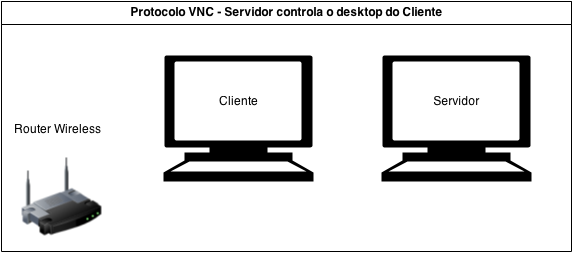
\includegraphics[width=100mm,scale=1]{vnc.png}
	\caption{Protocolo VNC}\label{fig:vnc}
	\end{figure}
	
	\textbf{Nota}: Rápido e eficaz numa rede local com boa largura de banda.
	
	
	
	
	\section{Resultados}
	

	
	Realizamos diversos testes de modo a colocar à prova o robô em diversas situações. 
	Acabámos por perceber que o robô detecta minas mesmo quando estas se encontram debaixo do solo. \\
	Por fim acabámos por testar
	o robô numa superfície em que garantimos que não existem quaisquer condutor. Fizemos isto poque,
	no sítio em que nos encontramos a trabalhar a instalação eléctrica foi toda feita pelo solo
	e como consequência o robô detecta minas em diversos sítios algo que é lógico dado que os campos magnéticos gerados 
	pelos cabos eléctricos vão interegir com o campo magnético do nosso sensor. Na figura \ref{fig:resultado} temos identificadas três minas,
	duas visíveis e uma enterrada e temos o robô na sua posição inicial. \\
	\tab A figura \ref{fig:resultado_final} foi tirada de um ângulo contrário à direção inicial do robô sendo que o mapa virtual obtido é o o mapa real 

	
	
	
	\begin{figure}[ht]
	  \centering
	  \begin{subfigure}{0.5\textwidth}
	    \centering
	    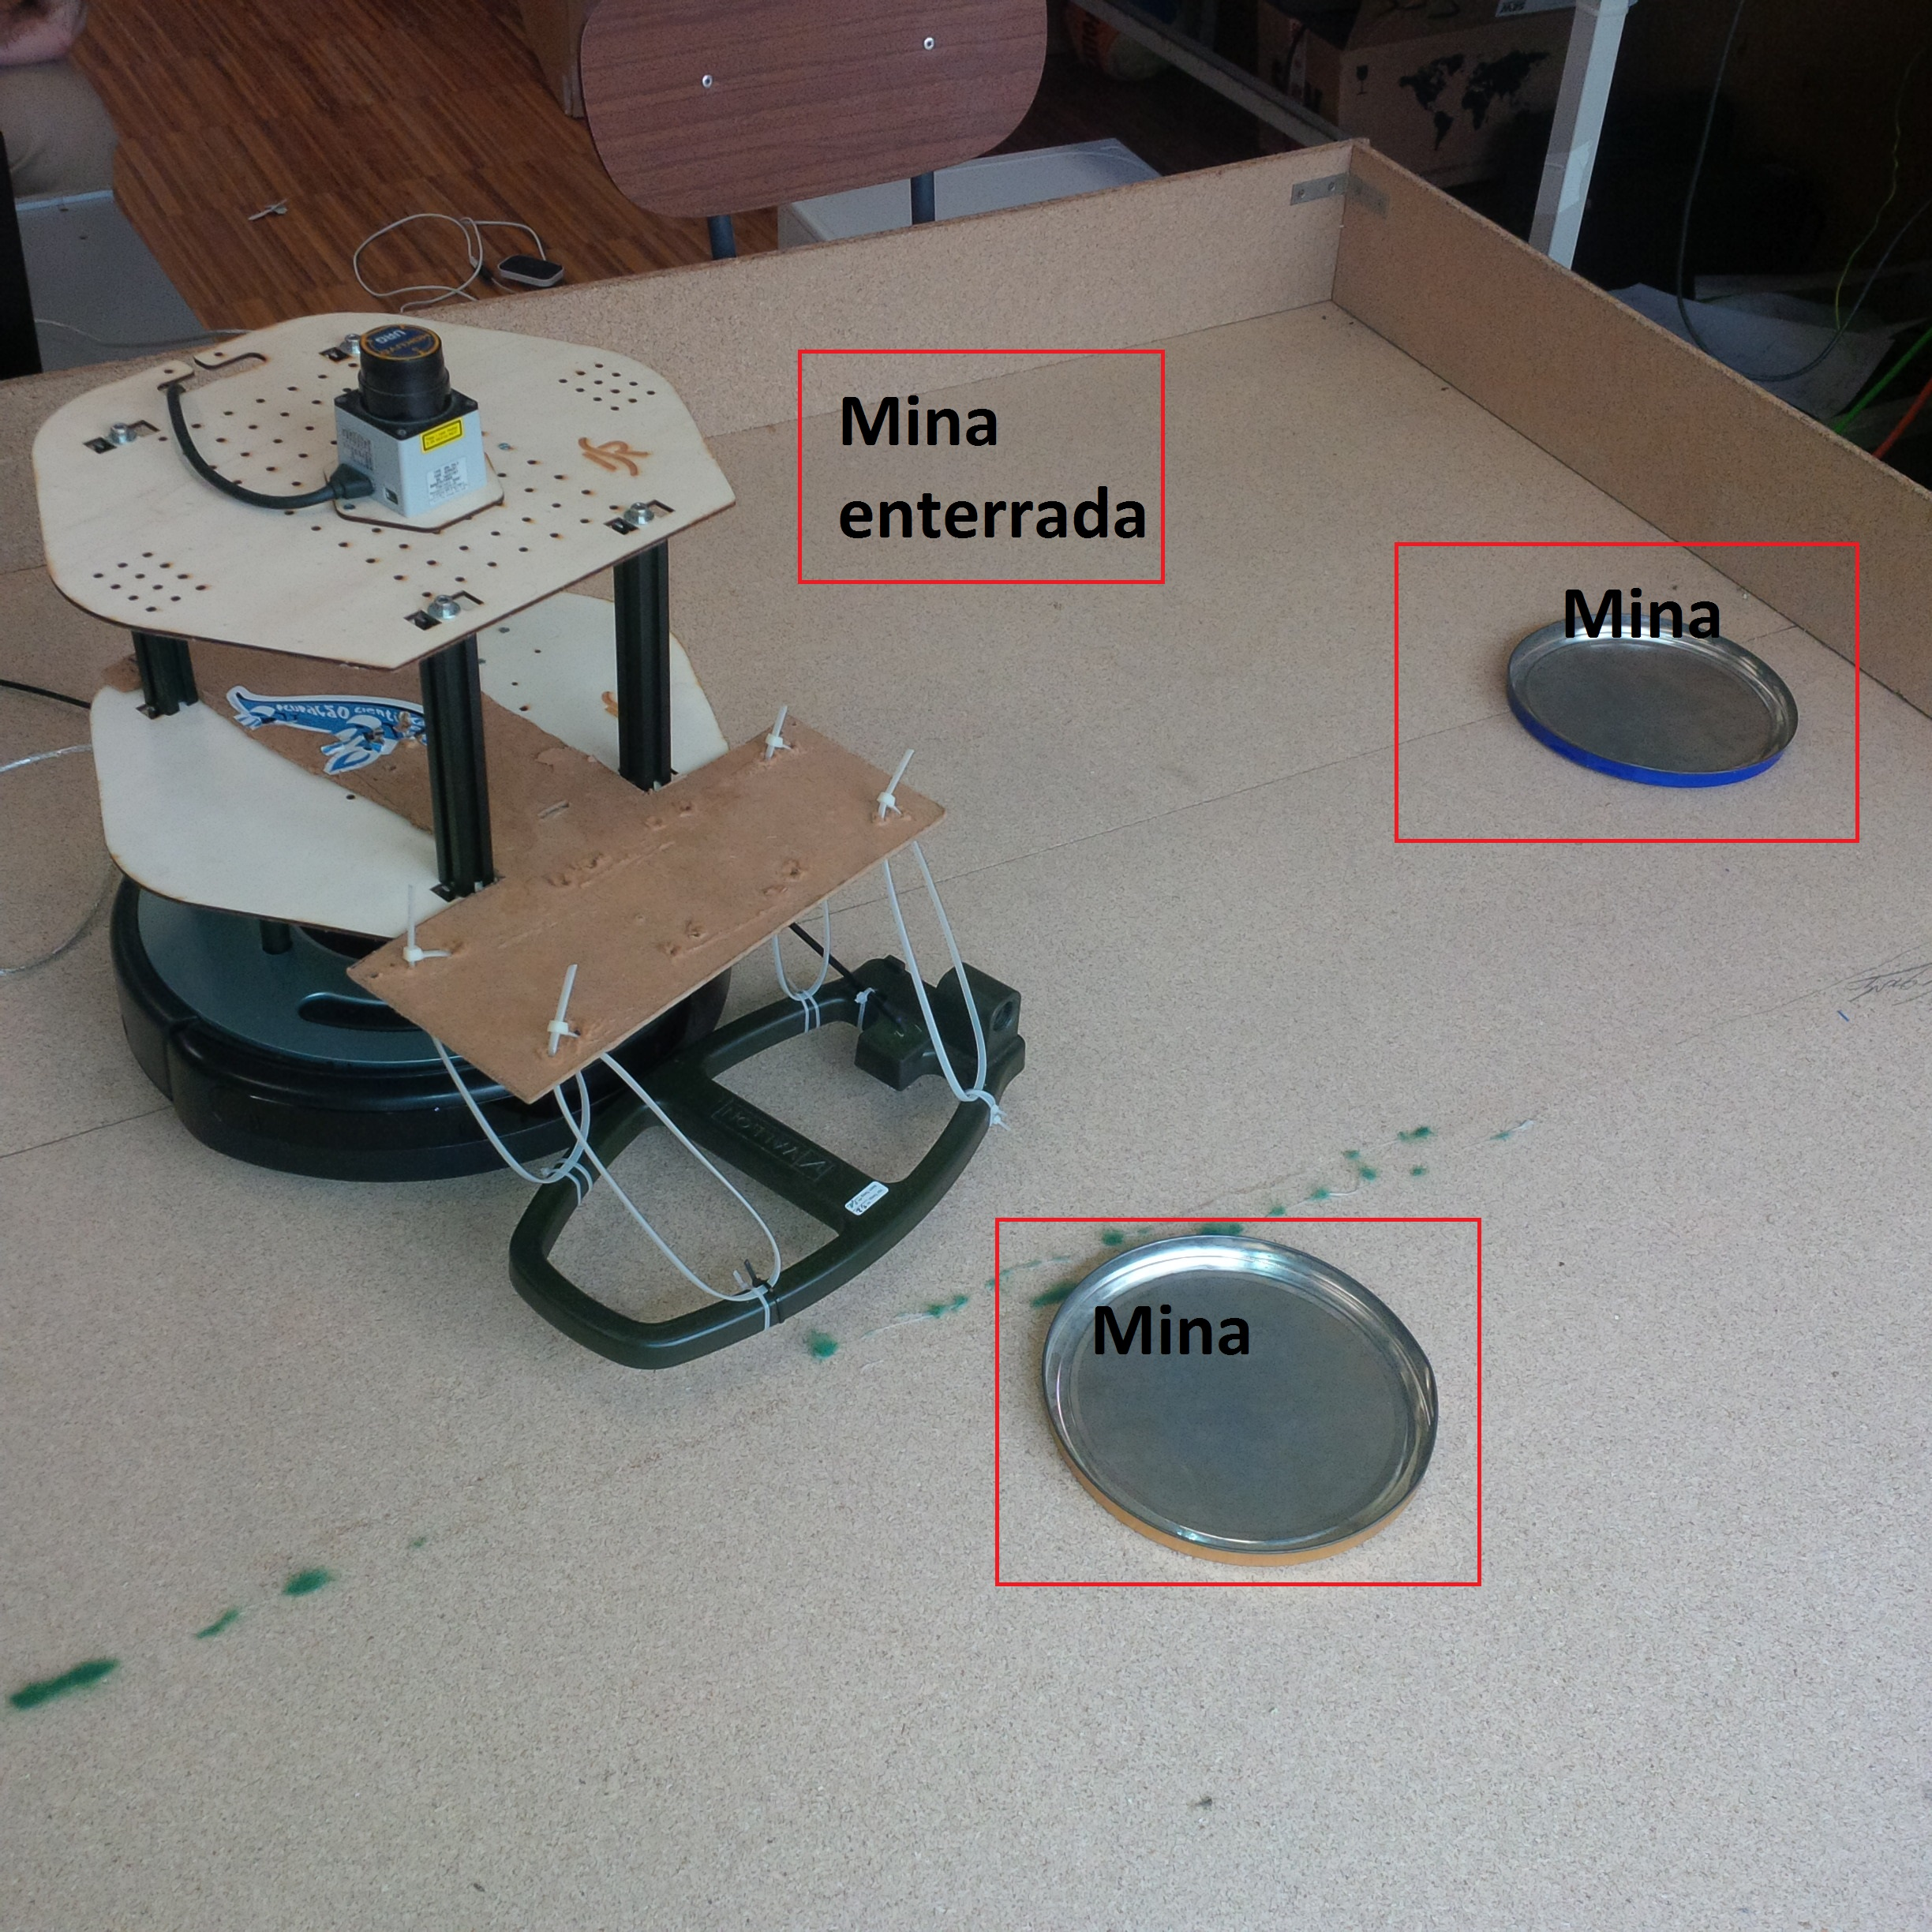
\includegraphics[width=70mm,scale=0.9]{teste_resultado.jpg}
	    \caption{Mapa real}
	    \label{fig:resultado}
	  \end{subfigure}%
	  \begin{subfigure}{0.5\textwidth}
	    \centering
	    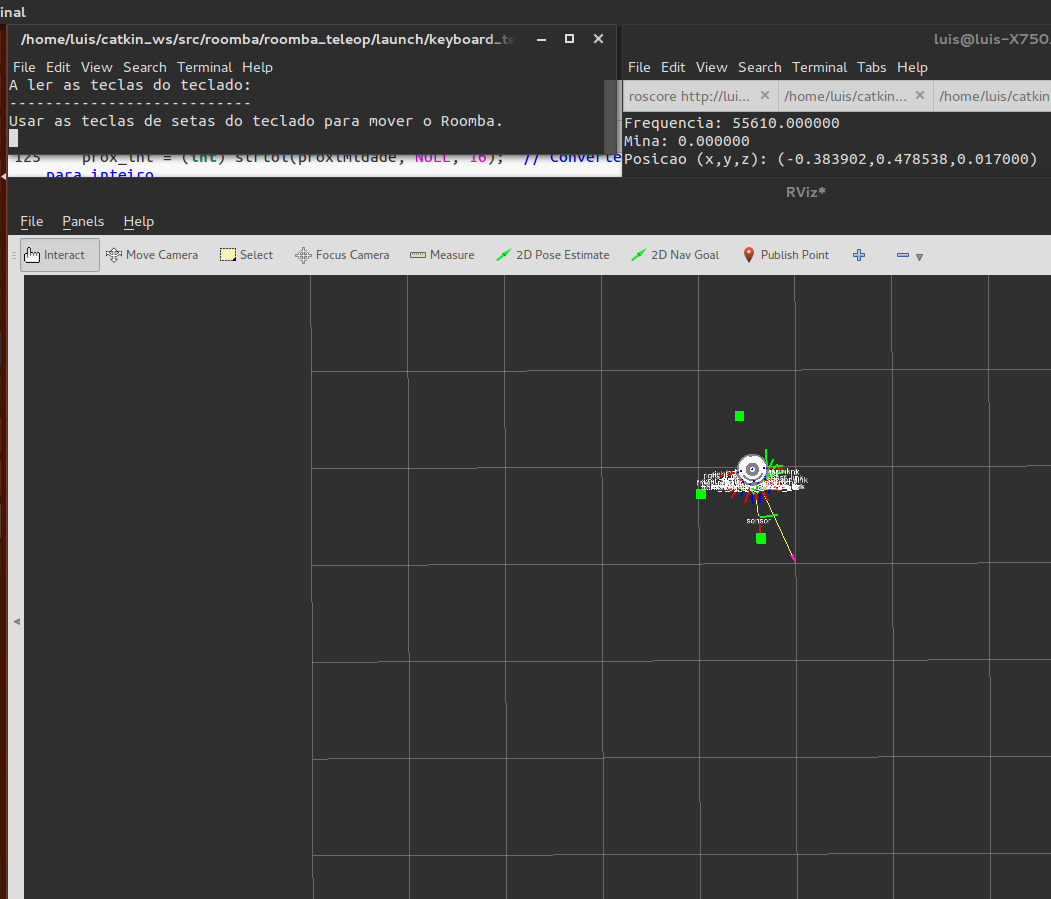
\includegraphics[width=80mm,scale=0.9]{teste.png}
	    \caption{Mapa virtual}
	    \label{fig:teste}
	  \end{subfigure}
	  
	  \caption{Teste para detecção de minas num labirinto}
	  \label{fig:resultado_final}
	  \end{figure}
	
	
	
	
	
	
	
	
	\section{Conclusões}
	

     \tab Com este projecto foi possível adaptar o robô ROOMBA para a deteção de minas com o auxílio do sensor LCD1000EVM. 
       Numa primeira parte do projecto foi criada a interface para que o sensor pudesse ser utilizado em Linux. Com o auxílio 
    da plataforma ROS (Robot Operatyng System) foi possível fazer a comunicação dos três periféricos ( computador, robô e sensor) esta plataforma permitiu ainda 
    criar o controlo por teclado da velocidade e direcção do robô. Por fim
    foi possível adaptar o sensor para uma bobine por nós desejada.\\ \tab Este projecto permitiu perceber a potencialidade tanto da plataforma ROS como do sensor LCD1000EVM. 
    A grande vantagem da plataforma ROS é que no futuro muito facilmente
    qualquer pessoa poderá adaptar este sensor a outros robôs ou outros sistemas robóticos, isto deve-se à vantagem do sistema de transformadas em que o ROS trabalha.
    O sensor LCD1000EVM tem a grande vantagem de com alguns pequenos passos se poder modificar e adaptar a qualquer bobine 
    que o utilizador pretenda, criando-se assim um sensor à medida do que o utilizador precisa.\\
    \tab Por fim foi conseguido utilizar o robô para a detecção de minas mesmo quando estas se encontram enterradas.


	
	
	
	
	

	

\bibliographystyle{plain}
\bibliography{mylib}
	
	\newpage
	
	  \section{Anexos}
	  
	  \subsection{Código C++}
	  \lstinputlisting{./code/c++.cpp}
	  
	  \newpage
	  
	  \subsection{Código Python}
	  \lstinputlisting{./code/python.py}
	  \newpage
	  
	
	\subsection{Código Matlab}
	  \lstinputlisting{./code/matlab.m}
	  
	  
	
\end{document}
